\documentclass[12pt]{article}
\usepackage[utf8]{inputenc}
\usepackage{amsmath, amssymb, physics, graphicx, tikz}
\usepackage[a4paper, margin=1in]{geometry}
\usepackage{fancyhdr}
\usepackage{hyperref}
\usepackage{tikz}
\usepackage{xcolor}
\definecolor{sectionrectanglecolor}{rgb}{0.25,0.5,0.75}
\definecolor{sectiontitlecolor}{rgb}{0.2,0.4,0.65}
\definecolor{subsectioncolor}{rgb}{0,0,0}
\definecolor{lightgray}{gray}{0.9}
\definecolor{darkgray}{gray}{0.1}
\definecolor{lightred}{rgb}{0.9,0,0.1}
\usepackage{wrapfig}
\usepackage{tcolorbox}

\newcommand{\be}{\begin{eqnarray}}
\newcommand{\non}{\nonumber \\ }
\newcommand{\ee}{\end{eqnarray}}
\newif\ifshowboardanswers
\showboardanswersfalse
% Set this to \showboardquestiontrue to include the end-of-lecture board question.
\newif\ifshowboardquestion
\showboardquestionfalse
\newcommand{\boardanswer}[1]{\ifshowboardanswers\\[0.35em]\textcolor{blue}{\textbf{Answer.} #1}\fi}

\fancyhead[L]{Special Relativity}
\fancyhead[R]{Lecture 9}

\title{\textbf{Lecture 9: Newtonian Dynamics Review (Forces, Energy, Momentum)}}
\author{Based on Morin's \textit{Introduction to Classical Mechanics}, Ch. 2.1/3.1-3.2/3.5/\\5.1/5.3/5.5-5.7}
\date{}

\begin{document}
\maketitle

\section*{Outline}
\begin{enumerate}
    \item \href{sec:statics}{Statics}
    \item \href{sec:Newton}{Using $F = ma$}
    \item \href{sec:Conservation}{Conservation of Energy and Momentum}
\end{enumerate}

\section{Statics}\label{sec:statics}
Before we start discussing dynamics and important conservation laws, let us briefly discuss statics. If an object is motionless and remains motionless, then Newton's second law ${\bf F} = m {\bf a}$ tells us that the total net force on that object must be zero. For any statics problem, it is thus perilous to identify all the relevant forces. In addition, because force is a vector (it has a direction), for any given problem, it is important to consider the right set of coordinates to solve the problem. 

Before we work out some examples, let us consider the different forces that typically play a role in many statics problems. 

\begin{itemize}
\item {\bf Tension: }Tension is the pulling force transmitted through a string, rope, cable, or similar object when it is pulled tight by forces acting from opposite ends. It always acts along the length of the object, directed away from the object on both sides. 

\item {\bf Normal Force:} The normal force is the support force exerted by a surface on an object resting on it. It acts perpendicular to the surface, balancing some or all of the object's weight. It can be thought of as the tension of a compressed spring.  

\item {\bf Friction:} Friction is the resistive force that opposes motion or the tendency of motion between two surfaces in contact. It acts parallel to the surface and opposite the direction of relative motion (or intended motion). Static friction concerns objects that are at rest relative to each other. The maximum force attributed to static friction $F =  \mu_s N$, with $\mu_s$ the coefficient of static friction and $N$ the normal force. Once the objects start moving w.r.t. another, this force should decrease. 

\item {\bf Gravity: }Gravity is the attractive force exerted by the Earth (or another massive body) that pulls objects toward its center, i.e., 
\be
F = m \frac{GM}{R^2}.
\ee
Near Earth’s surface, it gives objects weight and acts ``straight down" (directed towards the center of the Earth) with a magnitude of 
$F=mg$. 
\end{itemize}

Practically speaking, statics is the study of objects in equilibrium, meaning that they do not accelerate. This requires both the net force and the net torque to vanish:
\be
\sum {\bf F} &= 0, \\
\sum \tau &= 0.
\ee
Here $\tau = rF_\perp$ is the torque about a pivot, with $F_{\perp}$ the force perpendicular to the surface of the object and $r$ the distance from the pivot. Any static problem thus requires a careful consideration of all the forces and torques.  

\subsubsection*{Example 1: Block on a plane}
A block of mass $m$ rests on an incline at angle $\theta$ with coefficient of static friction $\mu_s$. Find a relation between $\mu_s$ and the angle of incline $\Theta$ for which the block remains at rest. 

Break down all the forces into components along the incline:
\begin{itemize}
  \item Gravity: $mg$ down.
  \item Normal: $N = mg \cos\theta$.
  \item Friction: $F_f$ up the incline.
\end{itemize}

Balancing the forces  along the incline of the plane:
\be
 F_f = mg \sin\theta.
\ee
But $|F_f| \leq \mu_s N = \mu_s mg \cos\theta$. Hence,
\be 
\tan\theta \leq \mu_s.
\ee
If $\mu_s = 1$, what is maximum angle $\theta$? Does that make sense?

\subsubsection*{Example 2: Block on a plane with horizontal force}

Next, we consider the same setup but now apply an additional force $F_a = mg$ as shown in Fig. 2.2 of Morin. We again have to collect all the forces. We now have an additional force that points in the direction of the friction (and thus carries a minus sign on the right-hand side): 
\be
F_f = mg \sin\theta - mg \cos \theta.
\ee
The normal force now has to counteract an additional downward force perpendicular to the inclined plane:
\be
N = mg \sin\theta + mg \cos \theta.
\ee
Again applying $|F_f| \leq \mu_s N$, we find 
\be
mg |\sin \theta - \cos\theta| \leq mg \mu_s (\cos \theta + \sin \theta).
\ee
Note that the absolute sign here was strictly introduced because the friction has to balance a force that could become negative. Now divide both sides by $mg\cos \theta$: 
\be
|\tan \theta - 1| \leq\mu_s (1 + \tan \theta).
\ee
Considering $\tan \theta \geq 1$, we find 
\be
\tan \theta \leq \frac{1+\mu_s}{1-\mu_s},
\ee
while for $\tan \Theta < 1$ we find 
\be
\tan \theta \geq \frac{1-\mu_s}{1+\mu_s},
\ee
or 
\be
\frac{1-\mu_s}{1+\mu_s}\leq \tan \theta \leq \frac{1+\mu_s}{1-\mu_s}. 
\ee
What happens when $\mu_s \rightarrow 0$? Does this make sense?

\subsubsection*{Example 3: Leaning ladder}
Let us now also fold in torque. A ladder of length $L$ and mass $m$ leans against a frictionless wall. If the static friction with the ground is $\mu_s$, what is the smallest angle the ladder can make with the ground and not slip (start moving)?

First, we identify all the forces. We have the friction of the ladder with the ground $F_f$, the normal pointing upward from the ground $N_1$, and the normal pointing sideways from the wall $N_2$. We have three equilibrium conditions now:
\be
\sum F_{\parallel} &=& 0, \\
\sum F_{\perp} &= &0. \\
\sum \tau  &=& 0.
\ee
where $\parallel$ means parallel to the ground and $\perp$ means perpendicular to the ground (and parallel to the wall). $N_1$ should balance the gravitational force of the ladder, i.e., $N_1 = mg$. At the same time, the normal force the wall exerts on the ladder should balance the friction, i.e., $N_2 =F_f$. So we have two relations and three unknowns. We need to use the balance of the torques.

We choose our pivot such that we end up with the least number of terms in the balancing of the torques. This point is determined by the point at which the largest number of forces are acting, since the force provides no torque around the point where it acts, since $r$ is zero. 

We have to project $N_2$ into the perpendicular component to the ladder, i.e., $N_2 \sin \theta$. The total torque around the pivot at the bottom of the ladder from $N_2$ is therefore given by $L N_2 \sin \theta$. Next, we compute the torque coming from gravity. Gravity acts on the center of mass of the ladder, which is in the middle of the ladder at $L/2$. Again, we have to consider the component that is orthogonal to the ladder, i.e., $m g (L/2) \cos \Theta $. Since these torques are in opposite directions, balancing the torques requires that
\be
N_2 L \sin \theta = m g (L/2) \cos \theta, 
\ee
or 
\be
N_2 = \frac{mg}{2 \tan \theta}
\ee
We know that $N_2 = F_f$ and the condition $F_f \leq \mu_s N_1 = \mu_s m g $, which leads to 
\be
\frac{mg}{2 \tan \theta} \leq \mu_s mg \rightarrow \tan \theta \geq \frac{1}{2\mu_s}.
\ee
What if you had chosen another pivot point? Consider the pivot point at the top of the ladder. The torque from gravity is the same as before. However, we now have to balance this against the torque from $N_1$ and from the friction $F_f$. Now we already know that $F_f = N_2$. So its torque should be identical (but opposite) to the scenario we considered above. In addition, we have the torque from $N_1$. This is given by the projection of the force component perpendicular to the ladder multiplied by the length of the ladder. The torques from gravity and from the friction point in the same direction, balancing the torque from $N_1$:
\be
m g (L/2) \cos \theta + N_2 L \sin \theta = N_1 L \cos \theta
\ee
Using $N_1 = mg$ we find 
\be
N_2 L \sin \theta = m g (L/2) \cos \theta,
\ee
which is the same as before (and we should thus obtain the same result for the $\theta$ in terms of $\mu_s$).

\section{Using ${\bf F} = m {\bf a}$}

How do objects move? From statics, we want to move to dynamics. Classical dynamics that is. This will allow us to talk about conservation laws and will set the stage of the next lecture, when we start discussing relativistic dynamics. 

Before Lagrange and Hamilton, we used forces as described by Newton's laws. 
Newton's laws are 
\begin{itemize}
\item {\bf First Law:} A body moves with constant velocity unless acted upon by a force. It also defines an initial reference frame, the frames we have discussed earlier, to which special relativity applies. Here, the definition of an inertial frame can be defined as a frame where Newton's first law applies.  
\item {\bf Second Law:} The time rate of change of the momentum of a body equals the force acting on the body. In classical mechanics (three) momentum is defined as ${\bf p} = m{\bf v}$ or ${\bf F} = m{\bf a}$, since ${\bf a} \equiv \frac{d{\bf v}}{dt}$. This law only holds in an inertial frame, as stated by the first law. It is not simply a definition of force, since some forces do not depend on the particles on which they act, but still, the rate of change of the momentum og these particles will be equivalent to the force. This law holds for all particles, i.e., if we act with the same force on two particles (of different or equal mass), the ratio of their acceleration is proportional to the ratio of their inverse masses.  
\item {\bf Third Law:} For every force on one body, there is an equal and opposite force on another body. Consider two particles with masses $m_1$ and $m_2$ that only interact with each other and nothing else. The total change in momentum is given by 
\be
\frac{d{\bf p}_{\rm total}}{dt} = \frac{d{\bf p}_{1}}{dt} + \frac{d{\bf p}_{2}}{dt} = {\bf F}_1 + {\bf F}_2 
\ee
with ${\bf F}_1$ and ${\bf F}_2$ the forces acting on the two masses. If the total momentum is conserved (assuming this is a fully isolated system), then ${\bf F}_1 = - {\bf F}_2$. In other words, we will never find a particle accelerating unless there is some other particle accelerating elsewhere. 
\end{itemize}
As Morin points out, these laws are of intellectual importance, but we should not attach too much significance to them. They are approximations of more fundamental theories, and we will see that the third law, for example, breaks down in special relativity, where (3) momentum is not conserved, even if there are only particles around and we have an isolated system\footnote{Some new form of momentum, which we call relativistic momentum, is conserved}. 

Using the second law, we can actually derive quantitative results. By means of collecting all forces of a given system, we can determine if that system is accelerating. We can distinguish two types of problems. The first concerns problems where we consider a physical situation, and as in the examples above, we have to collect all the forces, which generally act in different directions, and determine if an object is accelerating (there is a net force). The second set of problems concerns problems where the force is given as a function of, e.g., position, time, and velocity. We then have to solve a mathematical equality, i.e., by considering ${\bf F} = m {\bf a} = m \ddot{\bf x}$. For now, we will focus on the first of these problems. The second of these will be discussed in Diederik's lectures.  

To solve the first kind, it is useful to draw a diagram with all the forces. These are called free-body diagrams and should include all forces on the object(s) of interest. In the end, you will be able to write down a set of linear equations that can be solved (similar to dimensional analysis problems). 


\subsubsection*{Example 4: Atwood's Machine} 

Consider a pulley system with two masses $m_1$ and $m_2$. Both the strings and the pulleys are massless. What is the acceleration of the masses? And what is the tension in the string? 

First of all, the tension in the string should be the same everywhere; otherwise, there would be an infinite acceleration. The tension on $m_2$ should be $2T$, since there is zero net force on the massless pulley (again, otherwise there would be infinite acceleration). Using $F = ma$ we can thus write:
\be
T - m_1 g  = m_1 a_1, \\
2T - m_2 g = m_2 a_2.
\ee
We have two equations and three unknowns ($T$, $a_1$, and $a_2$). We need to find a relation between $a_1$ and $a_2$, which can be found by using the conservation of string. If we imagine $m_2$ moving by a distance $d$, then the total length of the string on this side of the pulley is reduced by $2d$. Therefore, $m_1$ has to go down by $2d$ to keep the length of the string the same. So the vertical position of the masses is related as $y_1 = -2 y_2$. Now taking two time derivatives to obtain the vertical acceleration, we find 
\be
a_1 = - 2 a_2. 
\ee
If we now combine this with the two equations above, we find 
\be
a_1 = g \frac{2m_2-4m_1}{4m_1+m_2}, \;\;\; a_2 = g \frac{2m_1-m_2}{4m_1+m_2}, \;\;\; T = \frac{3 m_1 m_2 g} {4 m_1 + m_2}.
\ee
Note that indeed $a_1$ and $a_2$ have the correct dimension (of acceleration) and tension $T$ is a force. If $m_2 = 2m_1$, then $a_1 = a_2 = 0$ and everything is at rest. If $m_2 \gg m_1$, we find $a_1 = 2g$ and $a_2 = -g$, i.e. $m_2$ is in free fall and $m_1$ gets accelerated upwards with $2g$. 

You can consider more masses and complicated pulleys, but deriving the forces will come down to a similar set of equations, where the final equations will always be to determine a relation between accelerations of the masses. See, for example, Q1 in M1 of 2023. 

\section{Conservation of Energy and Momentum}

Conservation laws are extremely important in physics. Within the context of classical / Newtonian Mechanics, they are derived from Newton's laws. It is therefore strictly not necessary to use them to solve a problem, but in many cases, it is much quicker to do so. We review conservation of energy and momentum, which is replaced by conservation of 4-momentum in special relativity (where (classical) energy and 3-momentum are not conserved). 

\subsection{Conservation of energy}

We start with Newton's second law:
\be
F = m a = m \frac{dv }{dt}. 
\ee
We can integrate the total force (see your calculus class):
\be
\int_{x_0}^{x} F(x') dx' &= &\int_{v_0}^{v} m v' dv' \nonumber \\
&= &\frac{1}{2} mv^2 - \frac{1}{2} m v_0^2.  
\ee
By equating $E =\frac{1}{2} m v_0^2 $, we then write 
\be
E = \frac{1}{2} m v^2 - \int_{x_0}^{x} F(x') dx'.
\ee
We now define the potential energy:
\be
V(x) \equiv -\int_{x_0}^{x} F(x') dx',
\ee
and thus
\be
E = \frac{1}{2} m v^2 + V(x).
\ee
The first term on the RHS is the kinetic energy. The equation is true at all points in the particle's motion, the sum of the kinetic and potential energy is constant; the total energy is conserved.  

Note that for a particle undergoing a given motion, both $E$ and $V(x)$ depend on the arbitrary (boundary) choice $x_0$. Hence, only the difference between $E$ and $V(x)$ is relevant. We can consider the difference in potential and kinetic energy between two points:
\be
\frac{1}{2} mv^2(x_2) - \frac{1}{2} mv^2(x_1) = V(x_1) - V(x_2) = \int_{x_1}^{x_2} F(x') dx' \equiv {\rm (Work)}_{x_1 \rightarrow x_2}.
\ee
Here we define the work-energy theorem, which states that a change in the particle's kinetic energy between points $x_1$ and $x_2$ equals the work done on the particle between $x_1$ and $x_2$.

We can write the differential form for the potential energy as:
\be
F(x) = - \frac{dV}{dx}.
\ee
It is usually straightforward to obtain the force, given the potential. It may be harder to obtain $V(x)$ from a given force (at least a closed-form expression). 

\subsubsection*{Example 5: Gravitational Potential}
Consider two point masses (a mass without a physical size) of mass $M$ and $m$, separated by a distance $r$. Newton's law tells us the force between these two masses is given by 
\be
F(r) = -\frac{GMm}{r^2}.
\ee
We can compute the potential energy via:
\be
V(r) - V(r_0) = - \int_{r_0}^r \frac{-G M m}{r'^2} = \frac{-GMm}{r} + \frac{GMm}{r_0}.
\ee
We can choose $r_0 = \infty$ and we find:
\be
V(r) = \frac{-GMm}{r}. 
\ee
Next, consider the gravitational potential near the Earth's surface of mass $m$ at height $y$. If $R$ is the radius of Earth and $M$ is its mass, we can write 
\be
V(R+y) - V(R) = \frac{-GMm}{R+y} - \frac{-GMm}{R} = \frac{GMm}{R} \left(1-\frac{1}{1+y/R}\right). 
\ee
Assuming $y \ll R$, we can Taylor expand the fraction, and approximate this as
\be
\frac{GMm}{R}\left(1-(1-y/R)\right) = \frac{GMmy}{R^2}.
\ee
Next, we use $GM/r^2 = g$, and we find the familiar result $V = mgy$. \\

\noindent
{\bf Conservative Force}. If we define the work between two points $x_1$ and $x_2$ to be:
\be
W_{\rm total} = \int_{x_1}^{x_2} F_{\rm total} dx,
\ee
then the force is called conservative if the force only depends on position (or is constant). This theorem is true only for forces in one dimension. Only if the force is conservative can we talk about the associated potential energy (since we would like to be able to label each value of $x$ with a unique number $V(x)$. The gravitational force is an example of a force that is conservative, even in three dimensions. 
\\

\noindent
{\bf Work vs potential energy}.
The work-energy theorem is relevant to one particle. The general work-energy theorem states that the work done on a system by external forces equals the change in energy of that system. This could be kinetic energy, internal potential energy, and internal kinetic energy, such as heat:
\be
W_{\rm external} = \Delta K + \Delta V + \Delta K_{\rm internal}.
\ee
For a point particle, which has no internal structure, only the first term on the RHS remains, and we are back to the point particle version of the work-energy theorem. 

\subsubsection*{Example 6: Raising a book}
Suppose I raise a book at constant speed, such that the kinetic energy is constant. Let us consider the work-energy theorem for 
\begin{itemize}
\item Just the book. Both you and gravity are external forces, and there is no change in the energy of the book as a system in itself:
\be
W_{\rm you} + W_{\rm grav} = 0 \Leftrightarrow mgh + (-mgh) = 0.
\ee
\item The book and the Earth. You are now the only external force (since `gravity' is now part of the system). Gravity is now an internal force that produces a potential energy:
\be
W_{\rm you} = \Delta V_{\rm Earth-book} \Leftrightarrow mgh = mgh
\ee
\item The book, the Earth, and you. In this case, there are no external forces. The internal energy of the system changes because the Earth-book gravitational potential energy increases, while your potential energy decreases; you have to burn calories to lift the book at constant speed. So we have
\be
0 = \Delta V_{\rm Earth-book} + \Delta V_{\rm you} \Leftrightarrow 0= mgh + (-mgh). 
\ee
Since we can't assume the human body is not 100\% efficient, your potential energy would decrease more than $mgh$. That extra loss is converted into heat:
\be
0 = \Delta V_{\rm Earth-book} + \Delta V_{\rm you} +\Delta K_{\rm internal} \Leftrightarrow 0= mgh + (-mgh - \eta) + \eta.
\ee
\end{itemize}
The main point is that you can look at a setup in different ways, depending on what you pick as your system. Potential energy, in one way, might show up as work in another. The main point is that the total energy is conserved for a closed system.\\ 

\noindent
Let us now consider forces in three dimensions. We again assume forces that only depend on position, i.e., ${\bf F }={\bf F }({\bf r})$, since such forces are the only ones that we could expect to be conservative. We can write 
\be
{\bf F} \cdot d{\bf r} = m {\bf v}\cdot d {\bf v},
\ee
where we use the inner product. Here we have defined $d{\bf r} = (dx, dy ,dz)$ and $d{\bf v} = (dv_x, dv_y, dv_z)$. We can integrate this equation from point $(x_0, y_0, z_0)$ to point $(x,y,z)$:
\be
\int_{{\bf r}_0}^{\bf r} {\bf F}({\bf r'}) \cdot d{\bf r'} = \frac{1}{2}m|{\bf v}|^2-\frac{1}{2}m|{\bf v}_0|^2. 
\ee
Just as in the one-dimensional case, $E$ is just a constant of integration $E = \frac{1}{2} m v_0^2$. The integrations on the left-hand side does depend on the paths in three-dimensional space. In one dimension, there is only one way between, e.g., $x_0$ and $x$. In short, we write:
\be
\frac{1}{2}m v^2-\int_{\bf r_0}^{\bf r} {\bf F}({\bf r'}) \cdot d{\bf r'} = E. 
\ee
Defining the potential energy as:
\be
V({\bf r}) = -\int_{\bf r_0}^{\bf r} {\bf F}({\bf r'}) \cdot d{\bf r'},
\ee
we can write:
\be
E = \frac{1}{2} mv^2 + V({\bf r}).
\ee
The sum of the kinetic energy and the potential energy is constant. 

Now let's come back to conservative forces. In three dimensions, the necessary condition for force to be conservative is that the curl of the force is zero, i.e., $\nabla \times {\bf F} = {\bf 0}$, in that case, the force will be path independent, even in three dimensions. See Morin for proof. The simpler and quicker proof is provided on page 151. If indeed the force is conservative, the potential is uniquely defined. We can then write down the differential form:
\be
dV = -{\bf F}({\bf r}) \cdot d({r}) \equiv - (F_x dx + F_y dy + F_z dz).
\ee
At the same time, we can expand the differential of the potential as 
\be
dV = \frac{\partial V}{\partial x} dx + \frac{\partial V}{\partial y} dy + \frac{\partial V}{\partial z} dz,
\ee
and hence:
\be
F_{X} =- \frac{\partial V}{\partial X} \Rightarrow {\bf F}({\bf r}) = - \nabla V({\bf r}),
\ee
with $X = x,y,z$. In other words, the force is the gradient of the potential. Now we can take the curl of this, i.e. 
\be
\nabla \times {\bf F}({\bf r}) = -\nabla \times \nabla V({\bf r}) = 0,
\ee
since the curl of a gradient is identically zero.

\subsection{Conservation of Momentum}
Assume an isolated system of two particles. From Newton's second law, we have ${\bf F} = d{\bf p}/dt$. We can integrate the force against time (instead of against space, as we did for energy and work):
\be
\int_{t_1}^{t_2} {\bf F} dt = {\bf p}(t_2)-{\bf p}(t_1).  
\ee
This integral is called the impulse. If we invoke the third law ${\bf F}_{ab}=-{\bf F}_{ba}$ (read this as the force of $b$ on $a$, and vice versa), we can write:
\be
{\bf p}_a(t_2)-{\bf p}_a(t_1) = - ({\bf p}_b(t_2)-{\bf p}_b(t_1)). 
\ee
We thus find:
\be
{\bf p}_a(t_1)+{\bf p}_b(t_1) = {\bf p}_a(t_2)+{\bf p}_b(t_2). 
\ee
Hence, the total momentum of an isolated system is conserved. This is a vector equality and hence it is really a system (3) of equations, which are all conserved independently. 

The example above is for two particles, but can naturally be extended to a system of $n$ particles. We simply define the force of particle $j$ on particle $i$ as ${\bf F}_{ij}$ (where $i,j$ run from $1$ to $n$): 
\be
\int \Delta {\bf p}_i = \int \left(\sum_j {\bf F}_{ij}\right) dt.
\ee
The change in total momentum of all particles is 
\be
\Delta {\bf P} \equiv \sum_i \Delta {\bf p}_i = \int \left(\sum_{ij} {\bf F}_{ij}\right) dt. 
\ee
Due to Newton's third law, $\sum_{ij} {\bf F}_{ij} = 0$; all forces cancel in pairs, and hence the total momentum of the system is conserved. 

\subsubsection*{Example 6: Rocket motion}
Consider a rocket of initial total mass $M$. The rocket propels itself forward by ejecting mass backwards with speed $u$ relative to the rocket. Let $m$ be the rocket's mass at some later time. During a short interval $dt$, the rocket ejects a positive amount of mass $dm$, so its mass changes from $m$ to $m-dm$, while its speed changes from $v$ to $v+dv$. To first order, the ejected mass moves at speed $v-u$ in the original frame. There are no external forces, so the total momentum of the system is conserved. We can thus write:
\be
mv = (m - dm)(v+dv) + dm(v-u). 
\ee
Assuming $dm, dv \ll 1$, we can neglect all terms that are quadratic in these small fluctuations. We thus end up with:
\be
\int_{v_i}^{v_f} dv =  \int_{m_f}^{m_i} u \frac{dm}{m}.
\ee
Note that we had to switch the bounds of integration, because we are considering an integral with steps $-dm$. This leads to 
\be
v_f-v_i = u \ln \frac{m_i}{m_f}.
\ee
If the initial speed of the rocket is $v_i=0$ and its initial mass is $m_i=M$, we find $v=u\ln(M/m)$. We revisit this example for a relativistic photon rocket in Lecture 12.

\subsection{Center of Mass Frame}

When considering momentum, we have to assume a frame of reference, since velocities are frame-dependent. If momentum is conserved in one frame, it should also be conserved in another. It turns out that there is a reference frame that can be advantageous to use. We can pick a frame for which the total momentum of the system is zero. This is referred to as the center of mass frame. The total momentum of this system (of particles) is given by ${\bf P}  = \sum_i m_i {\bf v}_i$. Now we pick a frame $S'$ which is moving with velocity ${\bf u}$. We then write:
\be
{\bf u} = \frac{\bf P}{M} = \frac{\sum_i m_i {\bf v}_i}{M}.
\ee
Here $M = \sum_i m_i$. Thus the total momentum in the new frame $S'$: 
\be
{\bf P}' = \sum_i m_i {\bf v}_i' = \sum_i m_i\left({\bf v}_i - \frac{\bf P}{M}\right) = {\bf P} - {\bf P} = 0.
\ee
We can define the position of the center of mass:
\be
R_{\rm CM} \equiv \frac{\sum m_i {\bf r}_i}{M}.
\ee
The center of mass does not move with respect to the center of mass frame. We can therefore choose the center of mass to be the origin of the center of mass frame. If we take two derivatives with respect to time of the center of mass position vector and multiply by $M$, we find 
\be
M {\bf a}_{\rm CM} = \sum_i m_i {\bf a}_i = \sum_i {\bf F}_i  = {\bf F}_{\rm total}.
\ee
We can therefore treat the system of particles in the center of mass frame as a point particle, and simply apply $F = ma$ to this point mass. 


\subsubsection*{Example 7: Two masses in 1-D}
Consider frame $S$. A mass $m$ with speed $v_m$ approaches a stationary mass $M$ ($v_M = 0$). The masses bounce off each other without loss of energy. What is the final velocity of these masses after the bounce? We can work in the center of mass frame. The total momentum in frame $S$ is $mv_m$. The center of mass frame $S'$ moves to the right with speed $mv_m/(m+M) \equiv u$. In this frame the velocity of the masses are $v'_m = v_m - u = Mv_m/(m+M)$ and $v_M' = 0 - u  = - mv_m/(m+M)$. In frame $S'$, the velocities of the masses should simply reverse after the bounce since energy is conserved. After this realization, we can move back to frame $S$, by adding $u$ to the new velocities in frame $S'$ after the bounce, i.e.,
\be
v_m &=& \frac{(m-M)v_m}{m+M}, \\
v_M &=& \frac{2m v_m}{m+M}.
\ee
\\

\noindent
{\bf Kinetic Energy} The relation between the kinetic energy of two frames $S$ and $S'$ where $S'$ is the center of mass frame is given by 
\be
K_S = K_{\rm CM} + \frac{1}{2} Mu^2,
\ee
where $K_{\rm CM}$ is the kinetic energy of the system in the center of mass frame, $\bf u$ is the velocity of frame $S'$ compared to frame $S$, and $M = \sum_im_i$. Therefore, $K$ in any frame equals the kinetic energy in the center of mass frame plus the kinetic energy of the entire system treated as a point particle of mass $M$ moving at the velocity of the center of mass frame $\bf u$. 

\subsection{Collisions}
We will consider elastic scattering only, for which kinetic energy is conserved. 

\subsubsection*{Example 8: Two masses in 1-D revisited}
We consider the same set-up as before. However, now we will work in a frame $S$ and explicitly use conservation laws before and after the bounce of the two masses. 

Conservation of momentum and kinetic energy tells us that:
\be
m v^i_m + 0  &=& mv_m^f + M v_M^f, \\
\frac{1}{2}m (v_m^i)^2 + 0 &=& \frac{1}{2} m (v_m^f)^2 + \frac{1}{2} M (v_M^f)^2. \label{eq:conservation}
\ee
We must solve these equations for the two unknowns $v_m^f$ and $v_M^f$. We can solve for $v_M^f$ first: 
\be
v_M^f = \frac{m}{M}(v_m^i - v_m^f),
\ee
and substituting that in the conservation of kinetic energy 
\be
m (v_m^i)^2 = m (v_m^f)^2 + \frac{m^2}{M}(v_m^i - v_m^f)^2. 
\ee
This leads to 
\be
\left( (m + M) v_m^f - (m-M)v_m^i\right)(v_m^f-v_m^i) = 0.
\ee
One solution is $v_m^f = v_m^i$. This satisfies the equations. In some sense, nothing really happens. The correct solution is the other root:
\be
v_m^f = v_m^i\frac{m-M}{m+M},
\ee
and using the expression for $v_M^f$ we get 
\be
v_M^f = \frac{2mv_m^i}{m + M},
\ee
consistent with our previous results. \\

In classical dynamics for one-dimensional elastic scatterings, the relative velocity of the two particles after the collision is the negative of the relative velocity before the collision. This can be directly shown using Eqs.~\eqref{eq:conservation} and assuming $v_M^i\neq 0$. We can rearrange those to find 
\be
m(v_m^i -v_m^f) &=& M (v_M^f - v_M^i), \\
m((v_m^i)^2 - (v_m^f)^2) &=& M ((v_M^f)^2 -(v_M^i)^2).
\ee
If we divide the second equation by the first, we find 
\be
v_m^i - v_M^i = -(v_m^f - v_M^f).
\ee
If you use this theorem along with the conservation of momentum, it allows you to solve the system also, and you would not get a quadratic equation. 

The above example is limited in scope. It only concerns one spatial dimension, and the number of problems that can be considered is minimal. To make things more interesting, we can consider interaction in two spatial dimensions. In that case, we need to be concerned with one additional momentum equation. Note that three spatial dimensions would be more of the same, since for many problems, one can find a frame of reference where the problem can be solved using only two spatial dimensions. 

\begin{figure}
\begin{center} 
\tikzset{every picture/.style={line width=0.75pt}} %set default line width to 0.75pt        

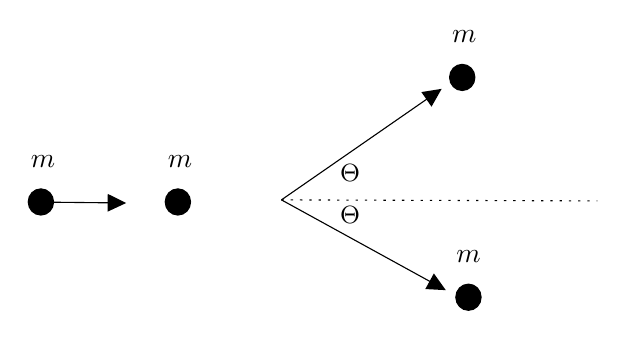
\begin{tikzpicture}[x=0.75pt,y=0.75pt,yscale=-1,xscale=1]
%uncomment if require: \path (0,300); %set diagram left start at 0, and has height of 300

%Flowchart: Connector [id:dp5958808506829039] 
\draw  [fill={rgb, 255:red, 0; green, 0; blue, 0 }  ,fill opacity=1 ] (88,130.7) .. controls (88,127.22) and (90.73,124.4) .. (94.1,124.4) .. controls (97.47,124.4) and (100.2,127.22) .. (100.2,130.7) .. controls (100.2,134.18) and (97.47,137) .. (94.1,137) .. controls (90.73,137) and (88,134.18) .. (88,130.7) -- cycle ;
%Straight Lines [id:da774514922768274] 
\draw    (88,130.7) -- (132.2,131.17) ;
\draw [shift={(135.2,131.2)}, rotate = 180.61] [fill={rgb, 255:red, 0; green, 0; blue, 0 }  ][line width=0.08]  [draw opacity=0] (8.93,-4.29) -- (0,0) -- (8.93,4.29) -- cycle    ;
%Flowchart: Connector [id:dp9275966313304485] 
\draw  [fill={rgb, 255:red, 0; green, 0; blue, 0 }  ,fill opacity=1 ] (154,130.7) .. controls (154,127.22) and (156.73,124.4) .. (160.1,124.4) .. controls (163.47,124.4) and (166.2,127.22) .. (166.2,130.7) .. controls (166.2,134.18) and (163.47,137) .. (160.1,137) .. controls (156.73,137) and (154,134.18) .. (154,130.7) -- cycle ;
%Flowchart: Connector [id:dp2448775352971747] 
\draw  [fill={rgb, 255:red, 0; green, 0; blue, 0 }  ,fill opacity=1 ] (291,70.7) .. controls (291,67.22) and (293.73,64.4) .. (297.1,64.4) .. controls (300.47,64.4) and (303.2,67.22) .. (303.2,70.7) .. controls (303.2,74.18) and (300.47,77) .. (297.1,77) .. controls (293.73,77) and (291,74.18) .. (291,70.7) -- cycle ;
%Flowchart: Connector [id:dp020775563565975985] 
\draw  [fill={rgb, 255:red, 0; green, 0; blue, 0 }  ,fill opacity=1 ] (294,176.6) .. controls (294,173.12) and (296.73,170.3) .. (300.1,170.3) .. controls (303.47,170.3) and (306.2,173.12) .. (306.2,176.6) .. controls (306.2,180.08) and (303.47,182.9) .. (300.1,182.9) .. controls (296.73,182.9) and (294,180.08) .. (294,176.6) -- cycle ;
%Straight Lines [id:da6654713491922019] 
\draw    (210,129.7) -- (284.73,77.91) ;
\draw [shift={(287.2,76.2)}, rotate = 145.28] [fill={rgb, 255:red, 0; green, 0; blue, 0 }  ][line width=0.08]  [draw opacity=0] (8.93,-4.29) -- (0,0) -- (8.93,4.29) -- cycle    ;
%Straight Lines [id:da4816667891850749] 
\draw    (210,129.7) -- (286.57,171.76) ;
\draw [shift={(289.2,173.2)}, rotate = 208.78] [fill={rgb, 255:red, 0; green, 0; blue, 0 }  ][line width=0.08]  [draw opacity=0] (8.93,-4.29) -- (0,0) -- (8.93,4.29) -- cycle    ;
%Straight Lines [id:da5822391697912397] 
\draw  [dash pattern={on 0.84pt off 2.51pt}]  (210,129.7) -- (362.2,130.2) ;

% Text Node
\draw (88,107) node [anchor=north west][inner sep=0.75pt]   [align=left] {$\displaystyle m$};
% Text Node
\draw (154,107) node [anchor=north west][inner sep=0.75pt]   [align=left] {$\displaystyle m$};
% Text Node
\draw (291,47) node [anchor=north west][inner sep=0.75pt]   [align=left] {$\displaystyle m$};
% Text Node
\draw (293,153) node [anchor=north west][inner sep=0.75pt]   [align=left] {$\displaystyle m$};
% Text Node
\draw (237,111.4) node [anchor=north west][inner sep=0.75pt]  [font=\small]  {$\Theta $};
% Text Node
\draw (237,131.4) node [anchor=north west][inner sep=0.75pt]  [font=\small]  {$\Theta $};


\end{tikzpicture}

\end{center}
\caption{Two billiard balls colliding after which they continue with an angle $\Theta$. }\label{fig:billiards}
\end{figure}

\subsubsection*{Example 9: Billiards}

Consider a (billiard) ball of mass $m_1$ and speed $v_1$. It collides with another billiard ball of mass $m_2$ that is at rest (see Fig.~\ref{fig:billiards}). The incoming ball gets deflected by an angle $\Theta$. We will use primes for the velocity components after the collision. We can use conservation of momentum in the $x$ and $y$ directions, and conservation of energy:
\be
m_1 v_1  &=& m_1 v_1' \cos \Theta + m_2 v_2' \cos \phi,\;\;\;\;(x-{\rm direction}) \\
0 &=& m_1 v_1' \sin \Theta - m_2 v_2' \sin \phi,\;\;\;\;(y-{\rm direction}) \\
\frac{1}{2} m_1 v_1^2 &=& \frac{1}{2} m_1 v_1'^2 + \frac{1}{2} m_2 v_2'^2. 
\ee
We will assume $m_1 = m_2 = m$. We must solve these equations for the three unknowns $v_1'$, $v_2'$, and $\phi$. We can square the momentum conservation equations and add them:
\be
m^2 v_1^2 &=& m^2(v_1' \cos \Theta + v_2' \cos \phi)^2 + m^2(v_1' \sin \Theta - v_2' \sin \phi)^2\nonumber \\
&=& m^2 (v_1'^2 + v_2'^2  + 2 v_1' v_2' \cos \Theta \cos \phi -2 v_1' v_2' \sin \Theta \sin \phi).
\ee
Now we also use that (from the unsquared momentum conservation equations)
\be
v_1' \sin \Theta = v_2' \sin \phi,
\ee
and 
\be
(v_1 - v_1'\cos \Theta) = v_2' \cos \phi,
\ee
to find 
\be
v_1^2 &=& v_1'^2 + v_2'^2 -2 v_1'^2 \sin^2 \Theta + 2 v_1'v_1\cos \Theta - 2 v_1'^2 \cos\Theta^2 \nonumber \\
&=& -v_1'^2 + v_2'^2 + 2v_1' v_1 \cos \Theta.
\ee
Reordered, this gives:
\be
v_1^2 - 2 v_1 v_1' \cos \Theta + v_1'^2 = v_2'^2.
\ee
We can use the conservation of kinetic energy to find 
\be
v_1' = v_1 \cos \Theta,
\ee
and 
\be
v_2' = v_1 \sin \Theta.
\ee
From conservation of momentum in the $y$-direction, we then get 
\be
 \cos \Theta \sin \Theta = \sin \Theta \sin \phi \rightarrow \cos \Theta = \sin \phi,
\ee
i.e, $\phi = 90^{\circ} - \Theta$, in other words, the balls would bounce off at right angles. Note that the other solution is $\Theta = 0$ (since then $\sin \Theta = 0$). In that case, there is no collision. So in this set-up, we force there to be a non-zero angle, and in that case, for elastic scattering, the balls bounce off at right angles. We will reconsider this example for relativistic billiard balls. The above can also be solved in the center-of-mass frame, where the solution will be a little easier to obtain.   

\ifshowboardquestion
\section*{Board Question}
\begin{tcolorbox}[colback=blue!5!white]
A block of mass $m$ slides without friction with speed $u$ and collides elastically in one dimension with a stationary block of mass $2m$.
\begin{enumerate}
    \item Write down conservation of momentum and kinetic energy.
    \boardanswer{$mu=mv_1+2mv_2$ and $\frac12mu^2=\frac12mv_1^2+\frac12(2m)v_2^2$.}
    \item Solve for the two final velocities.
    \boardanswer{For a 1D elastic collision, $v_1=(m-2m)/(m+2m)u=-u/3$ and $v_2=2m/(m+2m)u=2u/3$.}
    \item Check your answer in the center-of-mass frame.
    \boardanswer{$V_{\rm CM}=u/3$. In the CM frame the velocities reverse; transforming back gives $v_1=-u/3$ and $v_2=2u/3$.}
    \item Which part of this solution will have to be modified in relativistic collisions?
    \boardanswer{Momentum and energy must be replaced by relativistic momentum and total energy; kinetic energy alone is not the conserved energy.}
\end{enumerate}
\end{tcolorbox}
\fi

\end{document}
